\DiaryEntry{Golomb Codes}{2021-05-18}{Coding}

The Golomb–Rice codes belong to a family of codes designed to encode integers with the assumption that the larger an integer, the lower its probability of occurrence. The simplest code for this situation is the unary code. Golum codes then extend / use unary codes.

\subsection{Unary Code}

The unary code for a positive integer $n$ is simply $n$ ones followed by a zero. Thus, the code for $4$ is $11110$, and the code for $7$ is $11111110$. The unary code is the same as the Huffman code for the semi-infinite alphabet $\{1, 2, 3, \ldots \}$ with probability model $P(k) = \frac{1}{2^k}$. Because the Huffman code is optimal, the unary code is also optimal for this probability model.

\subsection{Golomb Code}

Although the unary code is optimal in very restricted conditions, we can see that it is certainly very simple to implement. One step higher in complexity are a number of coding schemes that split the integer into two parts, representing one part with a unary code and the other part with a different code. An example of such a code is the Golomb code.

The Golomb code is actually a family of codes parameterized by an integer $m > 0$. In the Golomb code with parameter $m$, we represent an integer $n > 0$ using two numbers $q$ and $r$ as

\bee
n = qm + r
\eee

with

\bee
q = \left\lfloor \frac{n}{m} \right\rfloor, \qquad r = n - qm
\eee


In other words, $q$ is the quotient (and can take on values $0, 1, 2, \ldots$) and $r$ is the remainder (which can take on values $0, 1, \ldots, m-1$) when $n$ is divided by $m$. The Golomb code works as follows: The quotient $q$ is represented by the unary code of $q$. Representing $m$ is slightly more tricky: If $m$ is a power of two, we use the $\log_2 m$-bit binary representation of $r$. If $m$ is not a power of two, we could use $\lceil \log_2 m \rceil$; however, we can reduce the number of bits required by using the $\lfloor \log_2 m \rfloor$-bit binary representation of $r$ for the first $2^{\lceil \log_2 m \rceil} - m$ values and the $\lceil \log_2 m \rceil$-bit binary representation of $r + 2^{\lceil \log_2 m \rceil} - m$ for the rest of the values. This way the average number of bits required is less than if we had used a fixed-length code with $\lceil \log_2 m \rceil$ bits. This code is also called a \emph{truncated binary encoding} (see also \href{https://en.wikipedia.org/wiki/Truncated_binary_encoding}{Wikipedia}).

An example will make the encoding process clearer.

\paragraph{Example for $m=4$.} The following table shows the various values of the Golomb code for different values of $n$.

\vspace*{3mm}

\begin{tabular}{c|cc|cc|c}
  $n$ & $q$ & $r$ & $q$ unary & $r$ representation & codeword \\ \hline
  0 & 0 & 0 & 0 & 00 & 000 \\
  1 & 0 & 1 & 0 & 01 & 001 \\
  2 & 0 & 2 & 0 & 10 & 010 \\
  3 & 0 & 3 & 0 & 11 & 011 \\
  4 & 1 & 0 & 10 & 00 & 1000 \\
  5 & 1 & 1 & 10 & 01 & 1001 \\
      & & & $\cdots$ & & \\
  8 & 2 & 0 & 110 & 00 & 11000
\end {tabular}
  
\vspace*{3mm}

\paragraph{Example for $m=5$.} Here we have $\lfloor \log_2 5 \rfloor = 2$ and $2^{\lceil \log_2 5 \rceil}  - 5 = 3$; i.e. the first three values are encoded with two bits. From $\lceil \log_2 5 \rceil = 3$ and $r + 2^{\lceil \log_2 5 \rceil} - 5 = r+3$ we follow that we represent the remaining values of $r$ with three bits as $r+3$. The following table shows the various values of the Golomb code for different values of $n$.

\vspace*{3mm}

\begin{tabular}{c|cc|cc|c}
  $n$ & $q$ & $r$ & $q$ unary & $r$ representation & codeword \\ \hline
  0 & 0 & 0 & 0 & 00 & 000 \\
  1 & 0 & 1 & 0 & 01 & 001 \\
  2 & 0 & 2 & 0 & 10 & 010 \\
  3 & 0 & 3 & 0 & 110 & 0110 \\
  4 & 0 & 4 & 0 & 111 & 0111 \\
  5 & 1 & 0 & 10 & 00 & 1000 \\
        & & & $\cdots$ & & \\
  9 & 1 & 4 & 10 & 111 & 10111 \\
  10 & 2 & 0 & 110 & 00 & 11000
\end {tabular}
  
\vspace*{3mm}

The following Figure shows the code tree for this code.

\begin{figure}[H]
  \centering
  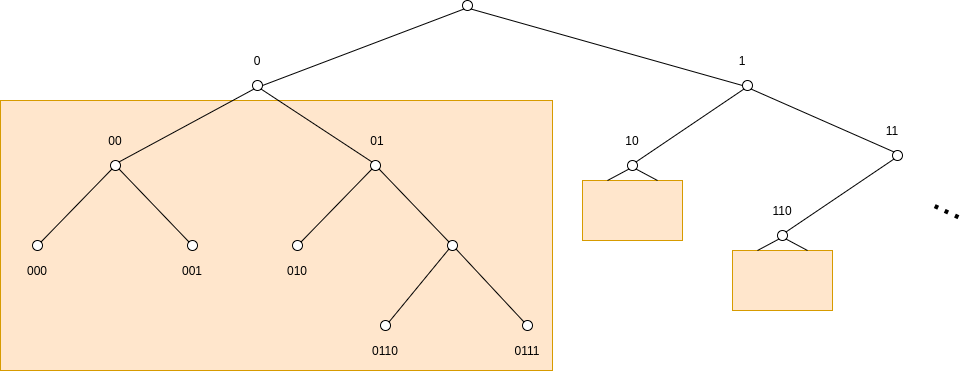
\includegraphics[scale=0.4]{images/2021-05-18-golomb_1.png}
\end{figure}

It can be seen that this is a prefix code as only the leaves correspond to codewords. The big orange block on the left corresponds to the encoding of $r$ ($2$ or $3$ bits) and the code continues to the right with more and more ones corresponding to the unary representation of $q$. The big orange block is replicated in the smaller orange ones.

\paragraph{Decoding.} We first decode $q$. If the codeword starts with a $0$ then discard the zero and contine with decoding $r$. Otherwise, count the number of ones followed by a zero which provides the unary representation of $q$ (the number of ones corresponds to $q$).

The next $2$ or $3$ bits correspond to the $r$-value (as shown in the orange box). From the table above it can be seen that the codes for $q$ with $3$ bits consist of an unassigned codeword of length $2$ (namely $11$) followed by a $0$ or $1$. From this follows the decoding rule: First read $2$ bits; if they encode a value less than $\lceil \log_2 5 \rceil = 3$, decoding is complete. Otherwise, read an additional bit and subtract $3$ from the result.

The decoding rule extends to other values of $m$.

%%% Local Variables:
%%% mode: latex
%%% TeX-master: "journal"
%%% End:
